\section{Simple distributed image reconstruction}\label{dist}
How do we distribute the major cycle. We need to distribute every ste, Gridding, FFT and Deconvolution.

Gridding, Large number of input data. This needs to be distributed
We use the Image domain gridding introduces in section \ref{hypo:idg} and use it as the basis for the distributed gridding.

The FFT is generally not worth distributing, if we can keep all the data in memory. When the gridding is done, in our setup, the grid is small enough to keep in memory. (cite distributed fftw)

Deconvolution is also worth distributing. CLEAN depending on the observation is the second most time consuming step. But gridding tends to be easier to distribute, so in some observations it is the most time consuming step.
Split the image into patches and deconvolve each patch.
Sadly not possible, we need communication. how we communicate is important.

We use a distributed Gridding and a distributed deconvolution. Which leads us to the following architecture.

\begin{figure}[h]
	\centering
	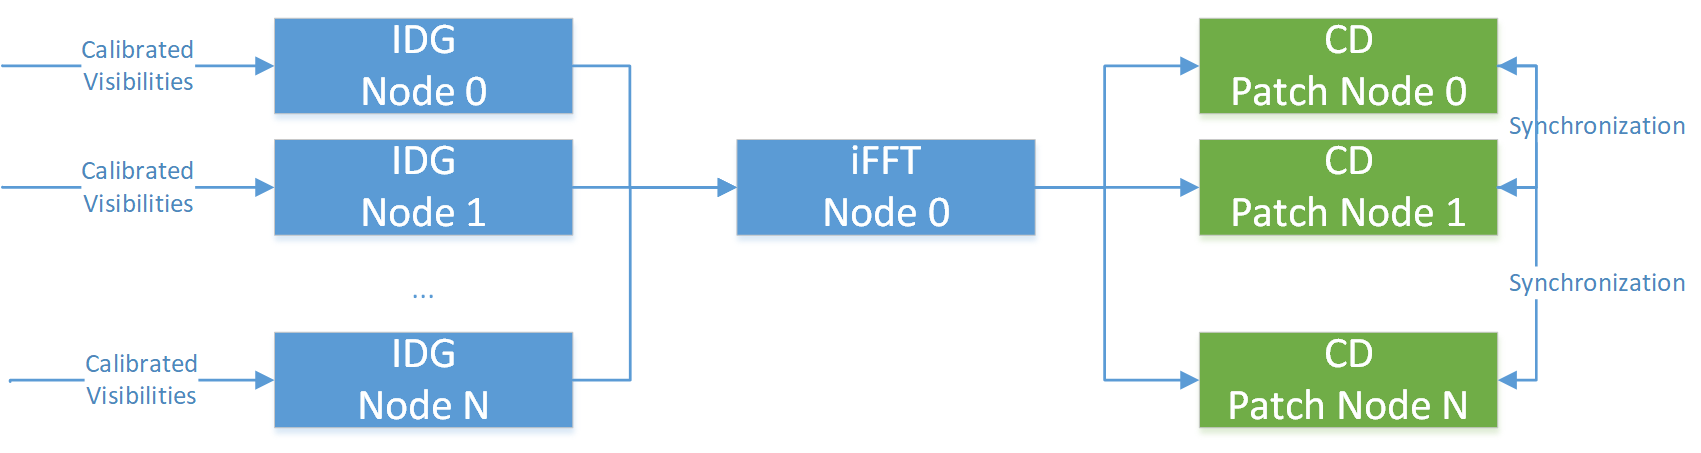
\includegraphics[width=0.80\linewidth]{./chapters/03.distribution/distributed_architecture.png}
	\caption{Distributed architecture for half a major cycle}
	\label{dist:architecture:fig}
\end{figure}

Where each node is one computer, i.e. has its own, possibly multiple cpus and its shared memory.
Split the input visibilities onto nodes. 
Do the gridding locally on each node
Communicate the grid
inverse FFT on one node.
Communicate the patches of the image.
Deconvolve each patch and communicate

How we distribute the IDG algorithm, and create a distributed deconvolution algorithm. Main contribution is the distributed deconvolution algorithm


\subsection{Distributing the IDG algorithm}\label{distribution:idg}




\subsection{Distributed deconvolution}
Main contribution
We start 


Coordinate Descent Algorithm why.

\subsubsection{Coordinate Descent Method}


Basic algorithm.


Implementation
Correlate the dirty image
Find max of objective
How to calculate a in -b/2a

Optimizations:
Why we only need to find the pixel which we can modify the most.

\subsubsection{ElasticNet Regularization}
L2 norm was used in other work. \cite{Ferrari}


Formula

\begin{figure}[h]
	\centering
	\begin{subfigure}[b]{0.3\linewidth}
		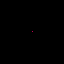
\includegraphics[width=\linewidth]{./chapters/03.distribution/L1.png}
		\caption{Effect of the pure L1 norm ($\lambda$ = 1.0) on a single point source.}
		\label{dist:cd:elastic:L1}
	\end{subfigure}
	\begin{subfigure}[b]{0.3\linewidth}
		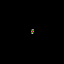
\includegraphics[width=\linewidth]{./chapters/03.distribution/L2.png}
		\caption{Effect of the pure L2 norm ($\lambda$ = 1.0) on a single point source.}
		\label{dist:cd:elastic:L2}
	\end{subfigure}
	
	\caption{Effect of the L1 and L2 Norm separately.}
	\label{dist:cd:elastic}
\end{figure}


Effect

Implementation



May even speed up convergence for correlated pixel values compared to L1 or L2\cite{friedman2010regularization}. But was not investigated in this project

\subsection{Major Cycle convergence}
Putting it all together

We have the Minor Cycle, which is easy to converge.

Coordinate Descent Path optimization \cite{friedman2010regularization}
Danger that CD takes too many pixel into a Major Cycle. Lower bound per iteration, PSF sidelobe
  can still be too low, danger when many psf sidelobes overlap

\subsection{Test on MeerKAT data}

